\section{Xamarin.Android}
�hnlich wie bei Xamarin.iOS bietet Xamarin.Android die M�glichkeit native Android Apps mit Xamarin
zu erstellen. Xamarin.Android benutzt den sogenannten Just-In-Time (JIT) Compiler um eine
raffinierte Optimierung der App Performance zur Laufzeit zu erm�glichen. Eine Xamarin.Android App
ist eine native Android APK (siehe Abb. \ref{fig:abb19}). Xamarin bringt 100\% von Google�s Android API in C\#
mit.
Mit dem bereits erw�hnten automatischen Binding-Generator kann man Java Code, Frameworks und benutzerdefinierte
Control-Elemente in einer Xamarin App benutzen.\\Im Gegensatz zu Xamarin.iOS kann man
Xamarin.Android sowie auf Windows- als auch auf einem Mac-Rechner installieren. Au�er das
aktuelle Android SDK werden bei der Installation von Xamarin.Android auch alle andere ben�tigte
Komponenten mitinstalliert. Xamarin Studio, bzw. Visual Studio stellt einen Android Emulator zur
Verf�gung, mit dem man eine App debuggen kann.

Genau wie Xamarin.iOS Entwicklung der herk�mmlichen iOS Entwicklung sehr �hnlich ist, ist auch
Xamarin.Android fast identisch mit der nativen Android App Entwicklung. Anstatt Java wird C\#
benutzt, aber die Entwicklungsans�tze sind gleich. Es werden Activities benutzt und der Lebenszyklus einer Activity
entspricht dem einer Activity aus der Android App Entwicklung. Die Ressourcen werden auch analog
geordnet.
\\Gleich am Anfang, wenn man ein neues Projekt erstellt, sollte man folgende drei Sachen einstellen:
\begin{itemize}
  \item Target Framework - dieses API Level wird zur Kompilierzeit benutzt und legt das Framework
  fest, mit der die App erstellt werden soll.
  \item Minimum Android Version - spezifiziert die �lteste Android Version, die die App unterst�tzen
  soll. Wird zur Laufzeit benutzt.
  \item Target Android Version - spezifiziert die Android Version auf der die App laufen soll. Wird
  zur Laufzeit benutzt.
\end{itemize}
Die verwendeten SDKs m�ssen durch den Open Android SDK Manager von Xamarin Studio (bzw. Visual
Studio) installiert werden.\\Wie bei Xamarin.iOS, bietet Xamarin.Android einen Designer f�r das
Gestalten der Benutzeroberfl�che.
\begin{figure}[!h]
\centering
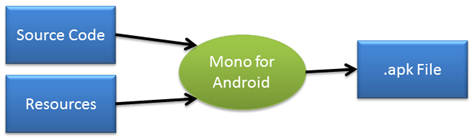
\includegraphics[scale = 0.8]{graphics/Xamarin_Android.png}
\caption{Xamarin.Android (Quelle:\cite{XamAndroid})}
\label{fig:abb19}
\end{figure}

\section{NuGet und Xamarin Component Store}
Xamarin bietet die M�glichkeit Komponente zu jeder App direkt aus der IDE hinzuzuf�gen.
Somit kann man diverse Controls, Web Service APIs und vieles mehr benutzen. Es k�nnen auch
popul�re Backends wie Microsoft Azure, Parse, Salesforce, SAP usw. in die APP integriert werden,
sowie auch Security Features wie Authentifizierung und Verschl�sselung.
 